\section{Constrained Black-Box Sequence Optimization Implementation Details and Results}
\label{app:sequence_opt}

This appendix provides implementation details for the constrained black-box sequence optimization experiments in Section~\ref{subsec:cpc_LLM_methods}. We describe the Ehrlich test functions used for evaluation (Section~\ref{subsec:ehrlich}), the procedure for training the safe policy via supervised fine-tuning on genetic algorithm data (Section~\ref{subsec:safe_policy_training}), the policy improvement procedure via DPO (Section~\ref{subsec:policy_improvement}), and supplementary results across additional risk levels (Figure~\ref{fig:extra_llm_policy_control_results}).

\subsection{Ehrlich Test Functions}
\label{subsec:ehrlich}

We evaluate CPC on Ehrlich functions \citep{chen2025generalists}, a class of synthetic test functions designed to capture the geometric structure of biomolecular sequence optimization problems such as antibody affinity maturation. An Ehrlich function $f: \mathcal{V}^L \rightarrow (-\infty, 1]$ maps sequences of length $L$ over a vocabulary $\mathcal{V}$ to a score indicating how well the sequence satisfies a collection of $c$ gapped motifs $\mathbf m^{(i)}$ with spacing $\mathbf s^{(i)}$. Formally,
\begin{align}
    f(\mathbf{x}) = \begin{cases}
        \prod_{i=1}^c g \circ h_q(\mathbf{x}, \mathbf{m}^{(i)}, \mathbf{s}^{(i)}) & \text{if } \mathbf{x} \in \mathcal{F} \\
        -\infty & \text{otherwise}
    \end{cases},
\end{align}
where $h_q$ measures motif satisfaction with precision $q$, $g$ is a response function capturing epistatic effects, and $\mathcal{F}$ is a feasibility set defined by a discrete Markov process with certain infeasible transitions (\textit{i.e.} some bigrams have zero probability mass). Sequences outside $\mathcal{F}$ are assigned $-\infty$, modeling expression constraints in real biophysical assays.

We follow the naming convention \textbf{Ehr(}$|\mathcal{V}|$\textbf{,} $L$\textbf{)-}$c$\textbf{-}$k$\textbf{-}$q$ from \citet{chen2025generalists}, where $k$ is the motif length and $q$ controls signal sparsity. Ehrlich functions are procedurally generated, have adjustable difficulty, and are provably solvable, making them well-suited for benchmarking constrained optimization algorithms. In our experiments, we use \textbf{Ehr(32, 32)-4-4-4}: sequences of length $L=32$ over a vocabulary of size $|\mathcal{V}|=32$, with $c=4$ motifs of length $k=4$ and quantization precision $q=4$.

\subsection{Training the Safe Policy}
\label{subsec:safe_policy_training}

Following \citet{chen2025generalists}, we initialize the optimization loop with a data package $\mathcal{D}^{(0)}$ collected from a genetic algorithm (GA) pre-solver. Starting from a single feasible seed sequence $\mathbf{x}_0$ sampled from the discrete Markov process, we run $n_0=10$ rounds of the GA with 5000 particles per iteration. This produces approximately 50K scored sequences that provide initial coverage of the feasible region $\mathcal{F}$. The GA uses mutation probability $p_m=0.05$ and survival quantile $\alpha=0.5$.

From the GA history, we construct the initial supervised fine-tuning (SFT) dataset by identifying improving pairs: for each sequence $\mathbf{x}$ in the history, we search for sequences $\mathbf{x}'$ within edit distance $\delta$ such that $f(\mathbf{x}') > f(\mathbf{x})$. These $(\mathbf{x}, \mathbf{x}')$ pairs form instruction-response examples for training the safe policy $\pi_{\theta_0}$, which we initialize from a Pythia 14M-parameter decoder-only transformer \citep{biderman2023pythia}. See Table~\ref{tab:sft_hyperparams} for hyperparameter settings.

\begin{table}[h]
\centering
\caption{Hyperparameters for training the safe policy via SFT.}
\label{tab:sft_hyperparams}
\begin{tabular}{ll}
\toprule
\textbf{Hyperparameter} & \textbf{Value} \\
\midrule
Base model & Pythia 14M \\
Learning rate & $10^{-6}$ \\
Training epochs & 10 \\
Batch size & 32 \\
Edit distance threshold ($\delta$) & $0.3 \cdot L$ \\
\bottomrule
\end{tabular}
\end{table}

\begin{algorithm}[t]
    \caption{Conformal Policy Control}
    \label{alg:cpc_round}
    \begin{algorithmic}
        \REQUIRE Safe policy $\pi_0$; context draws $\{X_i\}_{i=1}^n \sim p(X)$; target risk level $\alpha$
        \item[] \textbf{Phase 1: Safe Policy Data Collection}
        \STATE Draw actions $A_i \sim \pi_0(\cdot \mid X_i)$ for $i = 1, \ldots, n$
        \STATE Observe rewards $R_i = r(X_i, A_i)$ and losses $L_i = \ell(X_i, A_i)$
        \STATE Split data: $\mathcal{D}_{\text{train}}, \mathcal{D}_{\text{cal}} \gets \textsc{RandomSplit}(\{(X_i, A_i, R_i, L_i)\})$
        \item[] \textbf{Phase 2: Policy Improvement}
        \STATE $\pi_t \gets \textsc{ImprovePolicy}(\pi_0, \mathcal{D}_{\text{train}})$
        \item[] \textbf{Phase 3: Calibration}
        \STATE $\hat{\beta} \gets \textsc{CalibrateBeta}(\pi_0, \pi_t, \mathcal{D}_{\text{cal}}, \alpha)$ (Algorithm \ref{alg:calibrate_beta})
        \item[] \textbf{Phase 4: Constrained Deployment}
        \STATE Draw improved actions $A_i' \sim \pi_t^{(\hat{\beta})}(\cdot \mid X_i)$ via accept-reject for $i = 1, \ldots, n$
        \STATE \textbf{Return:} $\{A_i'\}_{i=1}^n$
    \end{algorithmic}
\end{algorithm}

\subsection{Improving the Safe Policy}
\label{subsec:policy_improvement}

To improve the safe policy, we take a fixed set of seed sequences from the GA optimizer history and sample actions from $\pi_{\theta_0}$. From the resulting data, we construct DPO preference triplets of the form $(\mathbf{x}, \mathbf{x}^+, \mathbf{x}^-)$, where $\mathbf{x}^+$ is preferred over $\mathbf{x}^-$ based on the oracle scores. We initialize the improved policy $\pi_{\theta_t}$ at the safe policy weights and train using the DPO loss \citep{rafailov2023direct}. See Algorithm \ref{alg:cpc_round} for pseudocode of a single round of CPC.

We chose DPO as our policy improvement method because \citet{chen2025generalists} demonstrated that it struggles with poor feasibility rates compared to other fine-tuning approaches, making it a challenging test case for our risk control procedure. See Table~\ref{tab:dpo_hyperparams} for hyperparameter settings.

\begin{table}[h]
\centering
\caption{Hyperparameters for policy improvement via DPO.}
\label{tab:dpo_hyperparams}
\begin{tabular}{ll}
\toprule
\textbf{Hyperparameter} & \textbf{Value} \\
\midrule
Learning rate & $10^{-7}$ \\
DPO $\beta$ & 0.4 \\
Training epochs per round & 1 \\
Batch size & 32 \\
Number of DPO rounds & 10 \\
\bottomrule
\end{tabular}
\end{table}

\begin{figure*}
    \centering
    \begin{subfigure}{\textwidth}
        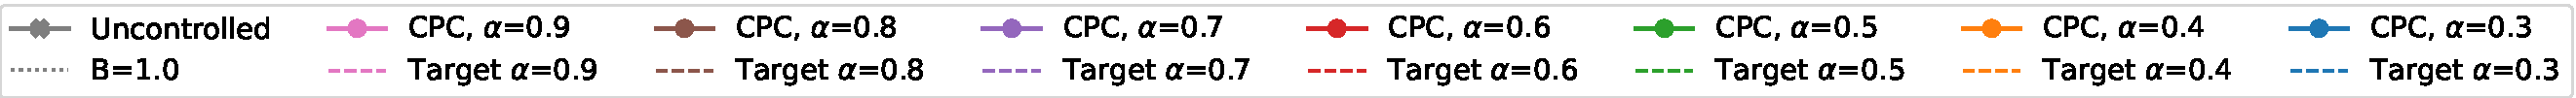
\includegraphics[width=\textwidth]{figures/legend_20251225_MixProp_fixedGetSeeds_0.2Hist_50minOld_solidErrsTrue_seeds0-9_8alphas.pdf}
    \end{subfigure}
    \\
    \begin{subfigure}{0.33\textwidth}
        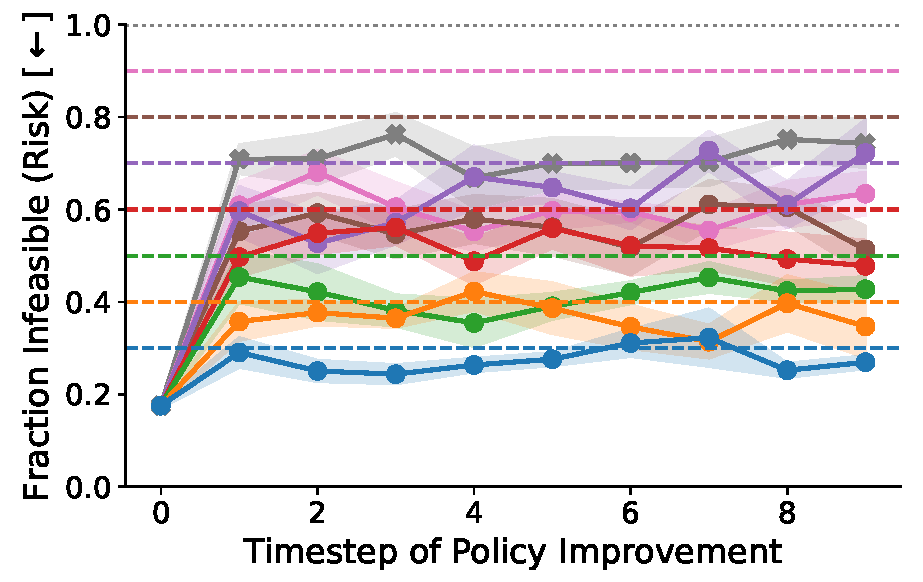
\includegraphics[width=\textwidth]{figures/Infeasibility_20251225_MixProp_fixedGetSeeds_0.2Hist_50minOld_solidErrsTrue_seeds0-9_8alphas_w24_h4.pdf}
    \end{subfigure}
    \hfill
    \begin{subfigure}{0.33\textwidth}
        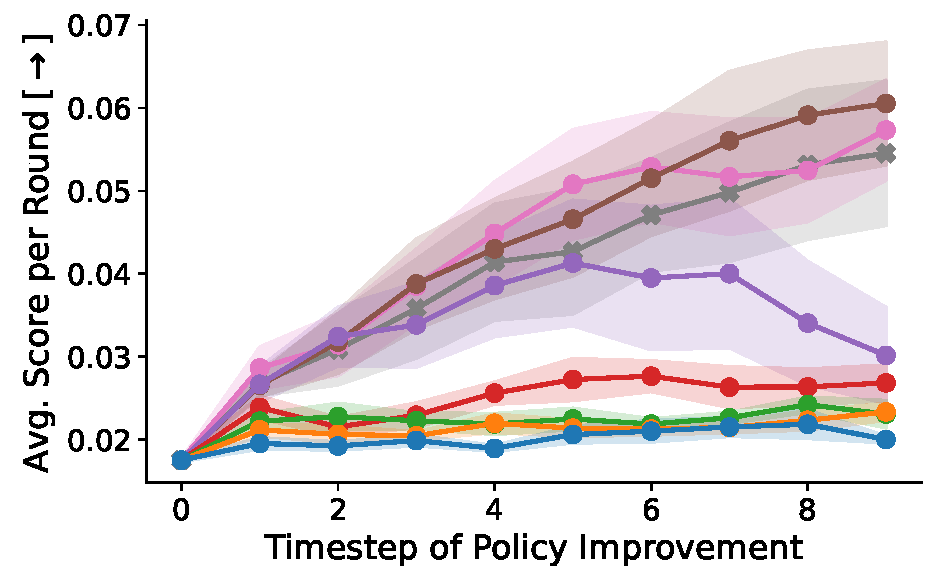
\includegraphics[width=\textwidth]{figures/AvgScores_20251225_MixProp_fixedGetSeeds_0.2Hist_50minOld_solidErrsTrue_seeds0-9_8alphas_w24_h4.pdf}
    \end{subfigure}
    \hfill
    \begin{subfigure}{0.33\textwidth}
        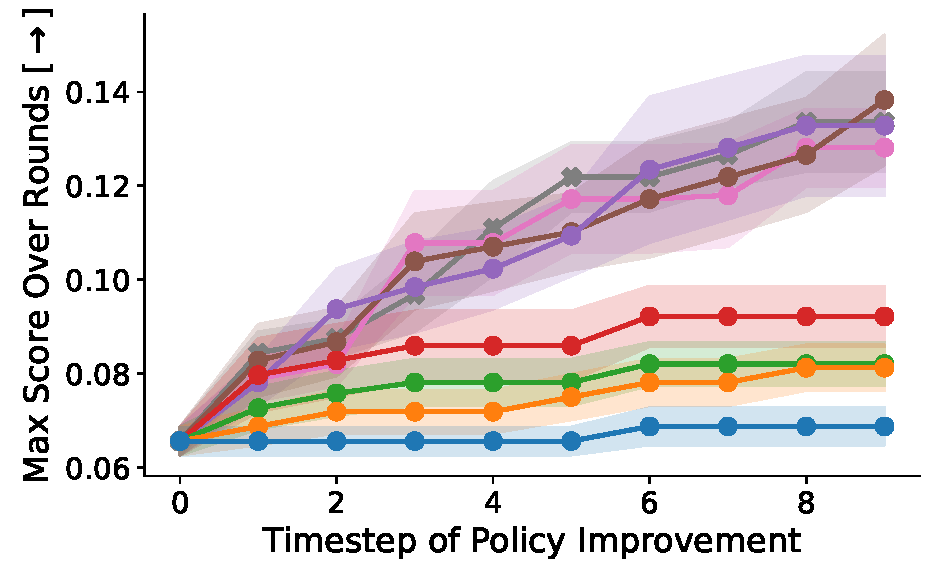
\includegraphics[width=\textwidth]{figures/MaxScores_20251225_MixProp_fixedGetSeeds_0.2Hist_50minOld_solidErrsTrue_seeds0-9_8alphas_w24_h4.pdf}
    \end{subfigure}
    \caption{
        Supplementary experimental results applying CPC to constrained black-box optimization of token sequences scored with Ehrlich functions. In the \textbf{left} panel, we show the average feasibility rate round-over-round. In the \textbf{center}, we show the average objective value of solutions sampled from the DPO-tuned policy, and in the \textbf{right}, the best solution found so far at each round. CPC allows us to easily modify the constraint violation risk by directly manipulating $\alpha$. We find that moderate risk control may actually stabilize the algorithm and lead to better overall performance since fewer samples are wasted to infeasibility constraints.
    }
    \label{fig:extra_llm_policy_control_results}
\end{figure*}

\clearpage
